\section*{A. Examples of Abelian Groups}

\begin{enumerate}

\item[1.]
\begin{equation}
x*y=x+y+k \text{ ($k$ is a fixed constant), on the set $\mathbb{R}$}
\end{equation}

\begin{enumerate}

\item[i]
$y*x=y+x+k=x+y+k=x*y$ \\
Commutative

\item[ii]
$x*(y*z)=x*(y+z+k)=x+(y+z+k)+k=x+y+z+2k=$ \\
$(x*y)*z=(x+y+k)*z=(x+y+k)+z+k=x+y+z+2k$ \\
Associative

\item[iii]
$x*e=x+e+k=x \text{, therefore } e=-k$ \\
$e*y=e+y+k=y \text{, therefore } e=-k$ \\
Identity is $-k$

\item[iiii]
$x*a=x+a+k=e=-k \text{, therefore } a=-x-2k$ \\
$a*x=a+x+k=e=-k \text{, therefore } a=-x-2k$ \\
Inverse is $-x-2k$

\end{enumerate}

\item[2.]
\begin{equation}
x*y=\frac{xy}{2} \text{, on the set} \{x \in \mathbb{R}:x \neq 0\}
\end{equation}

\begin{enumerate}

\item[i]
$y*x=\frac{yx}{2}=\frac{xy}{2}=x*y$ \\
Commutative

\item[ii]
$x*(y*z)=x*\frac{yz}{2}=\frac{x\frac{yz}{2}}{2}=\frac{xyz}{4}=$ \\
$(x*y)*z=\frac{xy}{2}*z=\frac{\frac{xy}{2}z}{2}=\frac{xyz}{4}$ \\
Associative

\item[iii]
$x*e=\frac{xe}{2}=x \text{, therefore } e=2$ \\
$e*y=\frac{ey}{2}=x \text{, therefore } e=2$ \\
Identity is $2$

\item[iiii]
$x*a=\frac{xa}{2}=e=2 \text{, therefore } a=\frac{4}{x}$ \\
$a*x=\frac{ax}{2}=e=2 \text{, therefore } a=\frac{4}{x}$ \\
Inverse is $\frac{4}{x}$

\end{enumerate}

\item[3.]
\begin{equation}
x*y=x+y+xy \text{, on the set} \{x \in \mathbb{R}:x \neq -1\}
\end{equation}

\begin{enumerate}

\item[i]
$y*x=y+x+yx=x+y+xy=x*y$
Commutative

\item[ii]
$x*(y*z)=x*(y+z+yz)=x+(y+z+yz)+x(y+z+yz)=x+y+z+xy+xz+yz+xyz=$ \\
$(x*y)*z=(x+y+xy)*z=(x+y+xy)+z+(x+y+xy)z=x+y+z+xy+xz+yz+xyz$ \\
Associative

\item[iii]
$x*e=x+e+xe=x \text{, therefore } e=0$ \\
$e*y=e+y+ey=y \text{, therefore } e=0$ \\
Identity is $0$

\item[iiii]
$x*a=x+a+xa=e=0 \text{, therefore } a=\frac{-x}{1+x}$ \\
$a*x=a+x+ax=\frac{-x}{1+x}+x+\frac{-x}{1+x}x=0=3$ \\
Inverse is $\frac{-x}{1+x}$

\end{enumerate}

\item[4.]
\begin{equation}
x*y=\frac{x+y}{xy+1} \text{, on the set} \{x \in \mathbb{R}: -1 < x < 1\}
\end{equation}

\begin{enumerate}

\item[i]
$y*x=\frac{y+x}{yx+1} =\frac{x+y}{xy+1} =x*y$ \\
Commutative

\item[ii]
$x*(y*z)=x*\frac{y+z}{yz+1}=\frac{x+\frac{y+z}{yz+1}}{x\frac{y+z}{yz+1}+1}=\frac{x y z + x + y + z}{x y + x z + y z + 1}=$ \\
$(x*y)*z=\frac{x+y}{xy+1}*z=\frac{\frac{x+y}{xy+1}+z}{\frac{x+y}{xy+1}z+1}=\frac{x y z + x + y + z}{x y + x z + y z + 1}$ \\
Associative

\item[iii]
$x*e=\frac{x+e}{xe+1}=x \text{, therefore } e=0$ \\
$e*y=\frac{e+y}{ey+1}=y \text{, therefore } e=0$ \\
Identity is $0$

\item[iiii]
$x*a=\frac{x+a}{xa+1}=e=0 \text{, therefore } a=-x$ \\
$a*x=\frac{a+x}{ax+1}=\frac{-x+x}{-x^2+1}=0$ \\
Inverse is $-x$

\end{enumerate}

\end{enumerate}

\section*{B. Groups on the Set $\mathbb{R}$ x $\mathbb{R}$}

\begin{enumerate}

\item[1.]
\begin{equation}
(a,b)*(c,d)=(ad+bc,bd) \text{, on the set } \{(x,y) \in \mathbb{R} x \mathbb{R}: y \neq 0\}
\end{equation}

\begin{enumerate}

\item[i]
$(c,d)*(a,b)=(cb+da,db)=(ad+bc,bd)=(a,b)*(c,d)$ \\
Commutative

\item[ii]
$(a,b)*((c,d)*(e,f))=(a,b)*(cf+de,df)=(adf+b(cf+de),bdf)=(adf+bcf+bde, bdf,) = $ \\
$((a,b)*(c,d))*(e,f)=(ad+bc,bd)*(e,f)=((ad+bc)f+bde,bdf)=(adf+bcf+bde, bdf)$ \\
Associative

\item[iii]
$(a,b)*(e_{1},e_{2})=(ae_{2}+be_{1},be_{2})=(a,b) \text{, therefore } (e_{1},e_{2})=(0,1)$ \\
$(e_{1},e_{2})*(a,b)=(e_{1}b+e_{2}a,e_{2}b)=(a,b) \text{, therefore } (e_{1},e_{2})=(0,1)$ \\
Identity is $(0,1)$

\item[iiii]
$(a,b)*(a',b')=(ab'+ba',bb')=(0,1) \text{, therefore } (a',b')=(\frac{-a}{b^2},\frac{1}{b})$ \\
$(a',b')*(a,b)=(a'b+b'a,b'b)=(0,1) \text{, therefore } (a',b')=(\frac{-a}{b^2},\frac{1}{b})$ \\
Inverse is $(\frac{-a}{b^2},\frac{1}{b})$

\end{enumerate}

\item[2.]
\begin{equation}
(a,b)*(c,d)=(ac,bc+d) \text{, on the set } \{(x,y) \in \mathbb{R} x \mathbb{R}: x \neq 0\}
\end{equation}

\begin{enumerate}

\item[i]
$(c,d)*(a,b)=(ca,da+b) \neq (ac,bc+d)=(a,b)*(c,d)$ \\
Not commutative

\item[ii]
$(a,b)*((c,d)*(e,f))=(a,b)*(ce,de+f)=(ace,bce+de+f)= $ \\
$((a,b)*(c,d))*(e,f)=(ac,bc+d)*(e,f)=(ace,(bc+d)e+f) $ \\
Associative

\item[iii]
$(a,b)*(e_{1},e_{2})=(ae_{1},be_{1}+e_{2})=(a,b) \text{, therefore } (e_{1},e_{2})=(1,0) $ \\
$(e_{1},e_{2})*(a,b)=(e_{1}a,e_{2}a+b)=(a,b) \text{, therefore } (e_{1},e_{2})=(1,0) $ \\
Identity is $(1,0)$

\item[iiii]
$(a,b)*(a',b')=(aa',ba'+b')=(1,0) \text{, therefore } (a',b')=(\frac{1}{a},\frac{-b}{b})$ \\
$(a',b')*(a,b)=(a'a,b'a+b)=(1,0) \text{, therefore } (a',b')=(\frac{1}{a},\frac{-b}{b})$ \\
Inverse is $(\frac{1}{a},\frac{-b}{b})$

A (non-Abelian) group

\end{enumerate}

\item[3.]
\begin{equation}
(a,b)*(c,d)=(ac,bc+d) \text{, on the set } \{(x,y) \in \mathbb{R} x \mathbb{R}\}
\end{equation}

\begin{enumerate}

\item[i]
$(c,d)*(a,b)=(ca,da+b) \neq (ac,bc+d)=(a,b)*(c,d)$ \\
Not commutative

\item[ii]
$(a,b)*((c,d)*(e,f))=(a,b)*(ce,de+f)=(ace,bce+de+f)= $ \\
$((a,b)*(c,d))*(e,f)=(ac,bc+d)*(e,f)=(ace,(bc+d)e+f) $ \\
Associative

\item[iii]
$(a,b)*(e_{1},e_{2})=(ae_{1},be_{1}+e_{2})=(a,b) \text{, therefore }  e_{1}=\frac{a}{a}$ \\
Since we can't divide by $0$, there is no general identity

\item[iiii]
No inverse without an identity element

\end{enumerate}

\item[4.]
\begin{equation}
(a,b)*(c,d)=(ac-bd,ad+bc) \text{, on the set } \mathbb{R} x \mathbb{R} \ \text{ with the origin removed}
\end{equation}

\begin{enumerate}

\item[i]
$(c,d)*(a,b)=(ca-db,cb+da)=(ac-bd,ad+bc)=(a,b)*(c,d)$ \\
Commutative

\item[ii]
$(a,b)*((c,d)*(e,f))=(a,b)*(ce-df,cf+de)$ \\
$=(a(ce-df)-b(cf+de),a(cf+de)+b(ce-df))$ \\
$=(ace-adf-bcf-bde, acf+ade+bce-bdf)=$ \\
$((a,b)*(c,d))*(e,f)=(ac-bd,ad+bc)*(e,f)$ \\
$=((ac-bd)e-(ad+bc)f,(ac-bd)f+(ad+bc)e)$ \\
$=(ace-bde-adf-bcf, acf-bcf+ade+bce)=$ \\
Associative

\item[iii]
$(a,b)*(e_{1},e_{2})=(ae_{1}-be_{2},ae_{2}+be_{1})=(a,b) \text{, therefore } (e_{1},e_{2})=(1,0)$ \\
Identity is $(1,0)$

\item[iiii]
$(a,b)*(a',b')=(aa'-bb',ab'+ba')=(1,0) \text{, therefore } (a',b')=(\frac{a}{a^2+b^2},\frac{-b}{a^2+b^2})$ \\
$(a',b')*(a,b)=(a,b)*(a',b')$ commutativity \\
Inverse is $(\frac{a}{a^2+b^2},\frac{-b}{a^2+b^2})$

\end{enumerate}

\item[5.]
The previous operation on the set $\mathbb{R} x \mathbb{R}$ is not a group because there is no identity or inverse for $(0,0)$, we'd have to divide by $0$ \\

\section*{C. Groups of Subsets of a Set}

\begin{enumerate}

\item[1]
$A+\emptyset=(A-\emptyset) \cup (\emptyset - A) = A \cup \emptyset = A$ \\
$\emptyset + B=( \emptyset - B) \cup (B - \emptyset ) = \emptyset \cup B = B$ \\
Identity element = $\emptyset$ (the empty set)

\item[2]
$A+A^{-1}=(A-A^{-1}) \cup (A^{-1}-A)=\emptyset \cup \emptyset$ \\
so $A-A^{-1}=\emptyset$,  $A^{-1}-A=\emptyset$ \\
and $A=A^{-1}$

\item[3]
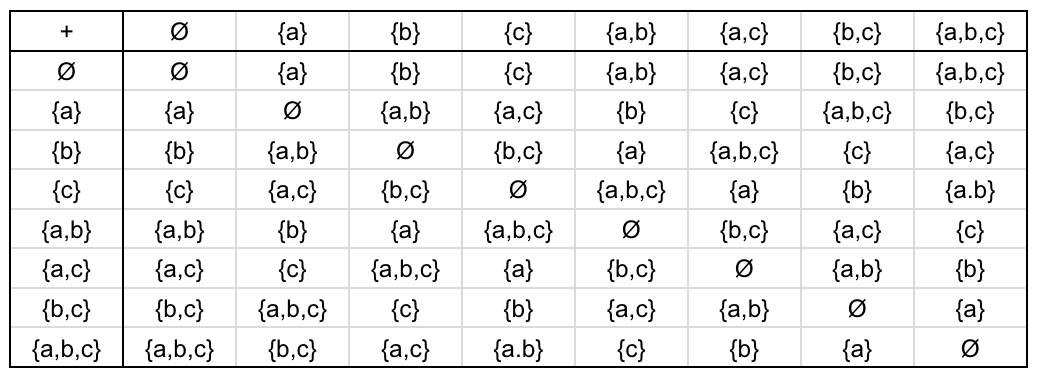
\includegraphics[scale=.6]{3_2_3}

\end{enumerate}

\section*{D. A Checkerboard Game}

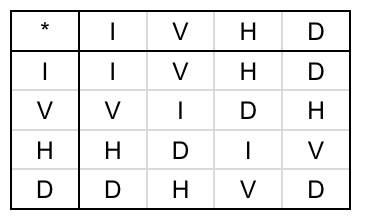
\includegraphics[scale=.75]{3_D}

\section*{E. A Coin Game}

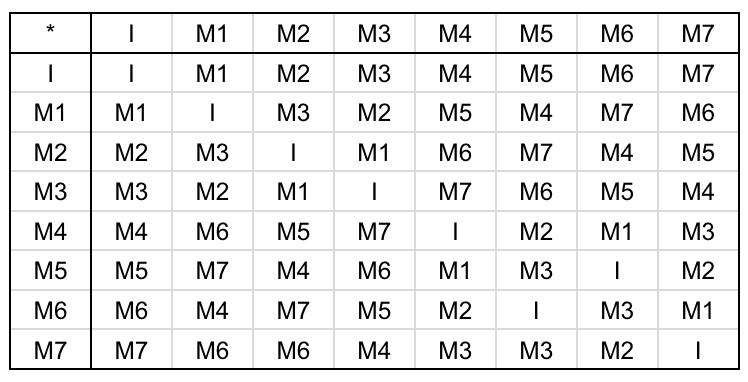
\includegraphics[scale=.75]{3_E}

$\langle G, * \rangle$ is a group because it has an identity element $I$ and for every value there is an inverse.

It is not commutative, you can tell because the top right and bottom left of the operation table are not transposes of each other. For example, $M_{7}*M_{6}=M_{2}$ but  $M_{6}*M_{7}=M_{1}$

\section*{F. Groups in Binary Codes}

\begin{enumerate}

\item[1]
$a_{n}+b_{n}=b_{n}+a_{n}$ for every n \\

\item[2]
$1+(0+1)=1+1=(1+0)+1$ \\
$1+(0+0)=1=(1+0)+0$ \\
$0+(1+1)=0+0=0=1+1=(0+1)+1$ \\
$0+(1+0)=1=(0+1)+1$ \\
$0+(0+1)=1=(0+0)+1$ \\
$0+(0+0)=0=(0+0)+0$ \\

\item[3]
$(a_1,...,a_n)+[(b_1,...,b_n)+(c_1,...,c_n)]$ \\
$=(a_1,...,a_n)+[(b_1+c_1),...,(b_n+c_n)]$ \\
$=(a_1+b_1+c_1),...,(a_n+b_n+c_n)$ \\
$=[(a_1+b_1),...,(a_n+b_n)]+(c_1,...,c_n)$ \\
$=[(a_1,...,a_n)+(b_1,...,b_n)]+(c_1,...,c_n)]$ \\

\item[4]
The identity is $0^n$, that is a word of length n where each element is 0. This way each element remains unchanged, as does the entire word. \\

\item[5]
The inverse of any element is itself. With no differences between the operands, the result of the operation is $0^n$ \\

\item[6]
$0+0=0=0-0$ \\
$1+0=1=1-0$ \\
$0+1=1=0-1$ \\
$1+1=0=1-1$ \\
$a_{n}+b_{n}=a_{n}-b_{n}$ \\

\item[7]
$1+1=0, 1=1+0$ \\
$1+0=1, 1=0+1$ \\
$0+1=1, 0=1+1$ \\
$0+0=0, 0=0+0$ \\

\end{enumerate}

\section*{G. Theory of Coding: Maximum-Likelihood Decoding}

\begin{enumerate}

\item[1]
$a_4=a_1+a_3, a_5=a_1+a_2+a_3$ \\
$000 \rightarrow a_4=0+0=0, a_5=0+0+0=0 $ \\
$001 \rightarrow a_4=0+1=1, a_5=0+0+1=1 $ \\
$010 \rightarrow a_4=0+0=0, a_5=0+1+0=1 $ \\
$011 \rightarrow a_4=0+1=1, a_5=0+1+1=0 $ \\
$100 \rightarrow a_4=1+0=1, a_5=1+0+0=1 $ \\
$101 \rightarrow a_4=1+1=0, a_5=1+0+1=0 $ \\
$110 \rightarrow a_4=1+0=1, a_5=1+1+0=0 $ \\
$111 \rightarrow a_4=1+1=0, a_5=1+1+1=1 $ \\

\item[2]
\begin{enumerate}
\item[a]
000000 \\
001001 \\
010111 \\
011110 \\
100011 \\
101010 \\
110100 \\
111101 \\

\item[b]
The minimum distance of $C_2$ is 2. \\
For example, 110100 + 111101 = 001001. \\

\item[c]
One error is sure to be detected. Two (or more) errors could lead to another code word.

\end{enumerate}

\item[3]
0000 \\
1001 \\
1110 \\
0111 \\

$x[0] = x[2]$ \\
$x[1] = x[2] + x[3]$ \\

Minimum distance = 2 \\

\item[4]
11111 $\rightarrow$ 11101\\
00101 $\rightarrow$ 00111\\
11000 $\rightarrow$ 11010\\
10011 $\rightarrow$ 10011\\
10001 $\rightarrow$ 10011\\
10111 $\rightarrow$ equidistant from 00111 and 10011\\

\item[5]
Every word will always differ in $m$ bits, so it would take at least $m$ bits to change one code word to another. Therefore, any number of bits smaller than $m$ cannot change a code word into another code word. If a code word has been changed and the result isn't another code word, we can easily detect this.

\item[6]
Let's say $x$ is less than $\frac{1}{2}(m-1)$ from both $a$ and $b$. \\
Then, the distance from $a$ to $b$ must be at most the distance from $x$ to $a$ plus the distance from $x$ to $b$: \\
$\overline{ab} \leq \overline{xa} + \overline{ba}$ \\
Plugging in for the distances from $x$ to $a$ and $b$: \\
$ \overline{ab} \leq \frac{1}{2}(m-1) + \frac{1}{2}(m-1) = (m-1)$ \\
Also, because both are code words we know $a$ and $a$ are at least $m$ distance apart: \\
$\overline{ab} > m$ \\
The distance from $a$ to $b$ can't satisfy both equations simultaneously: \\
$\overline{ab} \leq (m-1)$ and $\overline{ab} > m$ \\

\item[7]
The above shows that any word $x$ can only belong to one sphere (associated with the closest code word).

\item[8]
This claim is not true. \\
$t=\frac{1}{2}(m-1)=\frac{1}{2} < 1$ \\
Therefore, there exist some words that cannot be corrected because they are a distance of 1 from multiple code words.\\
\end{enumerate}

\end{enumerate}

